\documentclass[12pt]{report}%??????autres?choix?:?book,?report
\usepackage[utf8]{inputenc}%???????????gestion?des?accents?(source)
\usepackage[T1]{fontenc}%??????????????gestion?des?accents?(PDF)
\usepackage[english]{babel}%english gestion
\usepackage{hyperref}
\usepackage[bottom]{footmisc}
\usepackage[font=small,labelfont=bf]{caption}
\usepackage[newparttoc]{titlesec}
\usepackage[nonumberlist,toc]{glossaries}
\usepackage[export]{adjustbox}
\usepackage[margin=0.95in]{geometry}
\usepackage[square,sort,comma,numbers]{natbib}

%All the packages
\usepackage{lmodern,url,ragged2e,textcomp,lmodern,paralist}
\usepackage{graphicx,xcolor,float,afterpage}
\usepackage{chngcntr,csquotes,helvet,lastpage}
\usepackage{subcaption,wrapfig,fancyhdr,blindtext}
\usepackage{titletoc,transparent,datatool}

%List de mot ordonné
\newcommand{\sortitem}[1]{%
  \DTLnewrow{list}% Create a new entry
  \DTLnewdbentry{list}{description}{#1}% Add entry as description
}
\newenvironment{sortedlist}{%
  \DTLifdbexists{list}{\DTLcleardb{list}}{\DTLnewdb{list}}% Create new/discard old list
}{%
  \DTLsort{description}{list}% Sort list
  \begin{center}
	  \begin{inparaitem}%
    		\DTLforeach*{list}{\theDesc=description}{%
         \item \theDesc \hspace{0.1cm} }% Print each item
      \end{inparaitem}•%  
  \end{center}
}

%Nouvelles commandes
\renewcommand{\familydefault}{\sfdefault} %default font
\newcommand{\HRule}{\rule{\linewidth}{0.5mm}}
\newcommand{\Mline}{\hrule \mbox{}\\[0.1cm]}
\renewcommand{\thechapter}{\Roman{chapter}}

%final last page
\newcommand\blankpage{%
    \null
    \thispagestyle{empty}%
    \addtocounter{page}{-1}%
    \newpage}


%FORMAT DU CHAPITRE
\titleclass{\chapter}{straight}
\titleformat{\chapter}[hang]
  {}
  {\normalfont \sffamily \bfseries \thechapter.}
  {0pt}
  {\normalfont \sffamily \bfseries}
\titlespacing*{\chapter}{0pt}{50pt}{18pt}

%FORMAT De section
\renewcommand*\thesection{\arabic{section}}
\titleclass{\section}{straight}
\titleformat{\section}[hang]
  {}
  {\small \sffamily \bfseries \textit \thesection . }
  {0pt}
  {\small \bfseries \textit}
  
\titlespacing*{\chapter}{0pt}{50pt}{18pt}

%Comptage des figures
\renewcommand{\thefigure}{\arabic{figure}}

%Ne pas reset le numéro des figures  à chaque chapitre
\counterwithout{figure}{chapter}

%Custom footer and header
\pagestyle{fancy}
\fancyhf{}
%\lhead{Implement a Typing Speed Test With Qt}
\rhead{B00092351 Azarias Boutin, B00092354 Pierre Thubé}
\rfoot{Page \thepage}

\begin{document}

\begin{titlepage}
\begin{center}


% Title
\Mline
{ \LARGE Implement a Typing Speed Test With Qt \\[0.4cm] }
{ \LARGE Literature Review\\[0.4cm] }
\Mline
% Author and supervisor

\textsf{}\\[3cm]

\textsf{Boutin Azarias B00092351, B00092354 Pierre Thubé - Group 2\\[2cm]
BN013 BSC in Computing}


\end{center}
\end{titlepage}
\clearpage

\tableofcontents
\listoffigures
\chapter*{Keywords}
\begin{sortedlist}
  \sortitem{Keyboard}
  \sortitem{Keyboard layout}
  \sortitem{Fingers}
  \sortitem{Keys}
  \sortitem{Speed}
  \sortitem{Accuracy}
  \sortitem{Typing}
  \sortitem{Improvements}
  \sortitem{Learning}
\end{sortedlist}

\thispagestyle{empty}
\clearpage

\setcounter{page}{1}
\chapter{Abstract}
This review explores the way of improving the typing speed on the common keyboard.
Today's world is already full of keyboards, and it will never cease to increase. To be more efficient when using a computer, it is a good idea to learn how to type. On the web there are plenty of sources to improve your skills, but there is very little of them who really teach you how to type faster from scratch. The same goes for the existing software. And the main issue regarding this is that the software is not free.\\
The work presented here is based on books and websites that give advice on how to type speedily.\\
In order to address that issue, this review looks at the finger positions. Then it goes on to discuss how the user must practice to improve his or her typing skills. Lastly, it looks at the importance of accuracy and how this outweighs speed.

\clearpage
\chapter{Literature review}
\section{Some history}
In 1890, Lovisa Ellen Barnes wrote a book called "How To Become Expert in Typewriting"\cite{ref2} who was explaining how type on a Remington Typewriter.\\
In 1915, Dr. Henry Faulds wrote a book called "A Manual of Practical Dactylography"\cite{ref3}\\
An other example of book talking about dactylography.\cite{ref5}\\   
A more recent one published in 2012 and wrote by Faulds H.\cite{ref4}\\
As we can see, from a long time people provide way to learn how type so we can thereby say that way to type, and so typing speed, are always being important and are never been neglect by people.\\

\section{Keyboard}
The original layouts for the first mechanical typewriters were in alphabetical order (ABCDE etc..). Then different type of keyboard appeared according to languages used in each country (the most used is the QWERTY one but you can find AZERTY in France or QWERTZ in Germany for example).\\
Each of this layouts keyboard are classics one, that is mean when you buy a keyboard you will have one of this, but, since the invention of computers and indeed keyboards, a lots of research 	conducted to the invention of new non-classics layouts. Indeed, this new layouts had to made typing more easy and more comfortable. The most famous are Dvorak, Colemak and Workman.\\
Dvorak has been invented by August Dvorak and is the best alternative to QWERTY. It has been designed to increase typing speed, decrease errors and increase comfort.\\
After Dvorak, Colemak is the most popular. Also based on the QWERTY keyboard, it has been created in 2006 by Shai Coleman. It allow to promote the bearing of fingers on the middle rows of keys, it is better to maximise alternation between use right and left hands and minimize the movement of hands on the keyboard.\\
The third one is Workman. Thise one is less used than Dvorak and Colemak, but according with different developers, it is actually the best one to reduce fingers exhaustion. Indeed, it reduce usage of the two middle columns, reduce horizontal,diagonal and vertical finger stretching compared to Dvorak and Colemak.\cite{ref6}\\
To conclude about that, we can obviously say that from people have always trying to increase their typing skills by inventing new keyboards layouts which increase typing comfort and thus typing speed.     
\begin{figure}[h!]
   \begin{minipage}[b]{0.32\linewidth}
      \centering 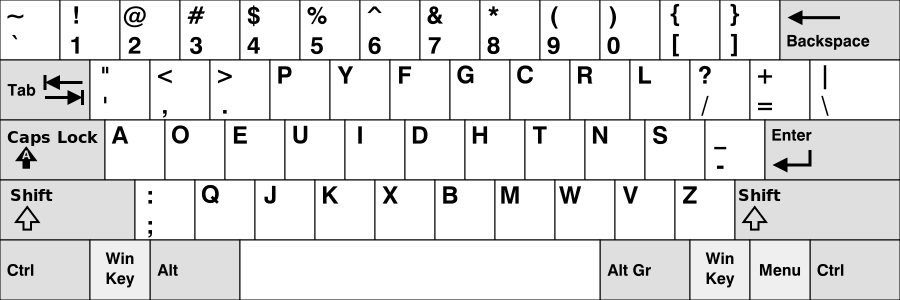
\includegraphics[scale=0.16]{images/KB_United_States_Dvorak.png}
      \caption{\it Dvorak Keyboard}
   \end{minipage}
   \begin{minipage}[b]{0.32\linewidth}   
      \centering 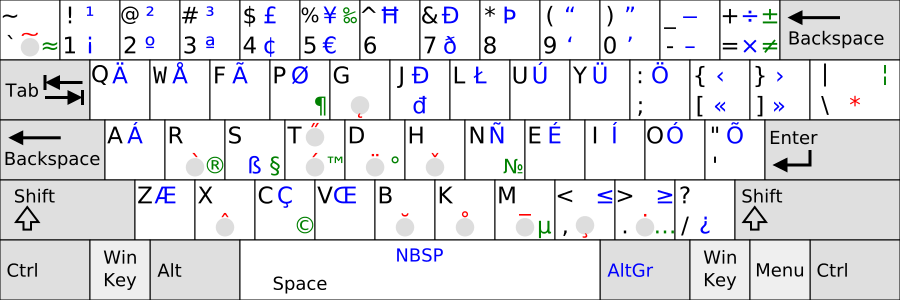
\includegraphics[scale=0.16]{images/KB_US-Colemak_with_AltGr.png}
      \caption{\it Colemak Keyboard}
   \end{minipage}
   \begin{minipage}[b]{0.32\linewidth}
      \centering 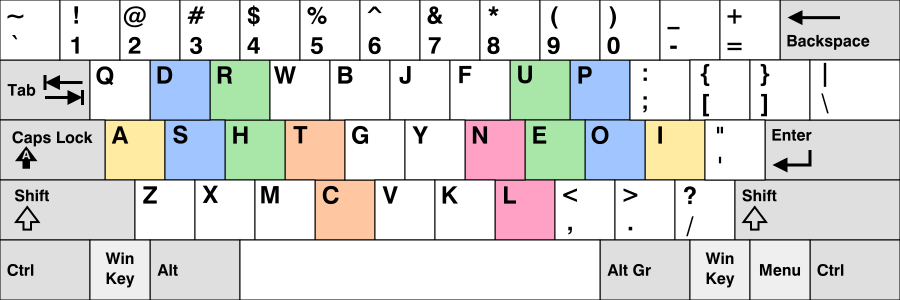
\includegraphics[scale=0.16]{images/KB_English_Workman.png}
      \caption{\it Workman Keyboard}
   \end{minipage}
\end{figure}
\clearpage

\section{Typing way and Fingers position}
To improve typing speed, in addition to change our keyboard, the only way is to practice. Actually, the average typing speed, calculate in Word Per Minute (WPM), is of 44 words.\cite{ref7} In the English language, the fastest typist in the world was Stella Pajunas who had a top speed of 216 words per minute. She realize it on a typewriter in 1946. Nowadays, it is easy with practice to had a typing speed of about 100 words par minute.\\ 
The typing way, which can be learn and improve on a lots of software and websites, is really the most important things to take in consideration to improve our typing speed. This typing way include the position of hands on a keyboard, which will change according to the type of keyboard, but for a QWERTY one it is like the figure 4 shows.
\begin{figure}[H]
\begin{center}
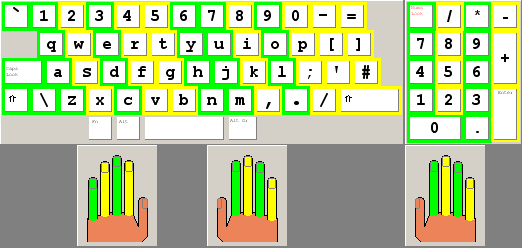
\includegraphics[width=9cm]{images/FingerHandPosUSA.png} 
\end{center}
\caption{\it Fingers position on QWERTY keyboard}
\label{Poulpy est multicolore}
\end{figure}
Here you can find some example of typing test on the internet:
\begin{itemize}
\item\it TypingTest.com\cite{ref8}
\item\it 10fastfingers.com\cite{ref9}
\end{itemize}
It also possible to find typing lessons on the internet.\\
To conclude about this part we can say that way to type and typing speed are things very democratize on the internet especially with a lots of website who can explain you best way to type, position of hands, give you advice and way to improve your typing style with speed test. That is showing that the development of a typing test is something useful.
Every book and website available regarding improving the typing speed are first mentions the finger positions.\\
As the book written by \citet{beginners}, the fingers must be positioned on the \textit{baseline}. The baseline, is the line on the keyboard containing the letters \textit{F} and \textit{J}. As with 'touch typing in ten lessons' \cite{tenlessons} book explains, every fingers should have an assigned letter. The figure below \ref{fing_pos} shows where the finger position is assigned on a QWERTY keyboard.
\begin{figure}[H]
	\centering
	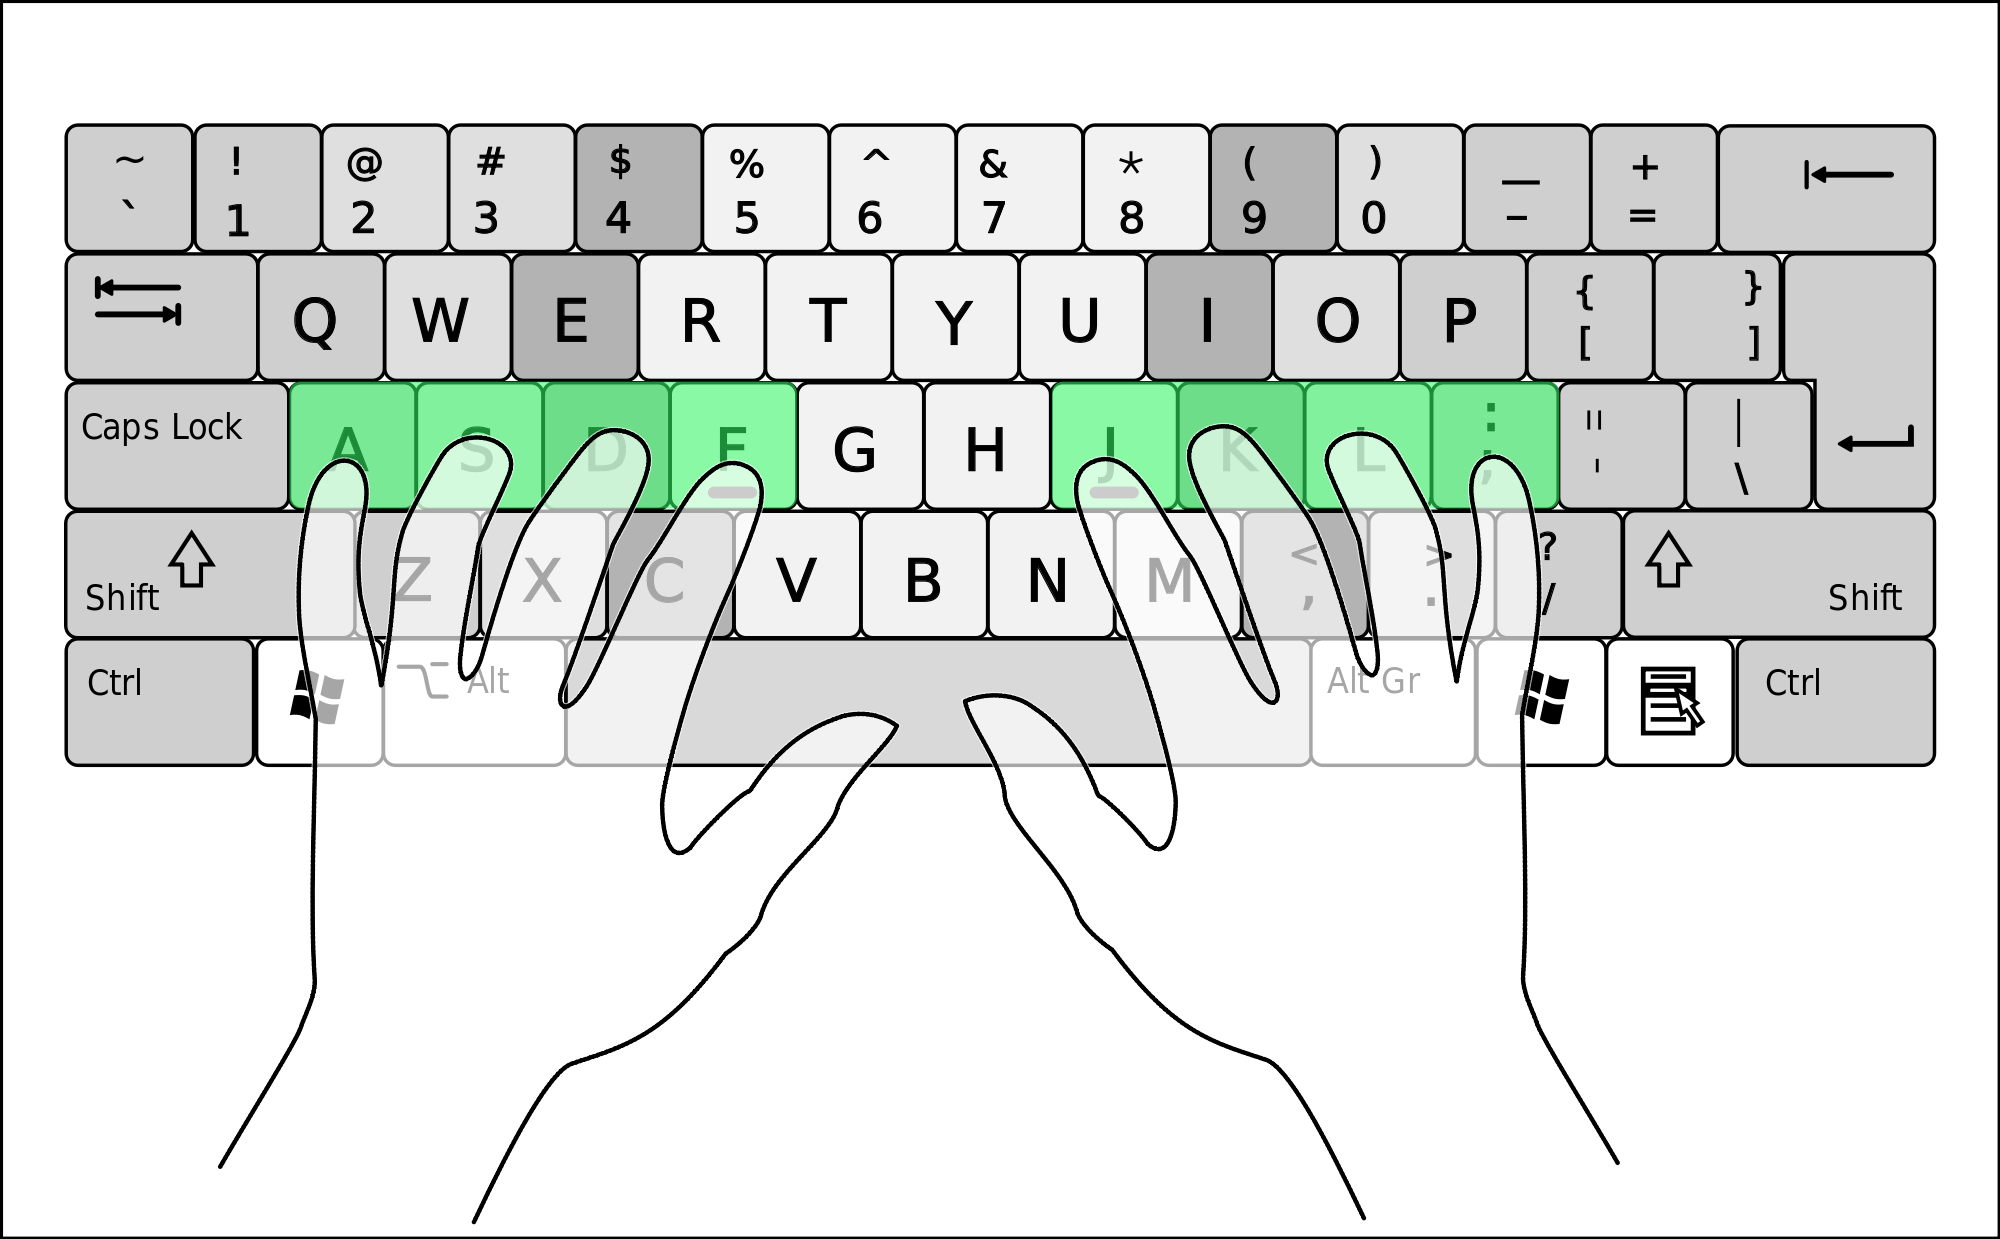
\includegraphics[width=0.7\textwidth]{images/fing_pos.png}
	\caption{Position of the fingers on a QWERTY keyboard}\label{fing_pos}
\end{figure}
However, the layout of the keyboard may vary but the finger position will stay on the same baseline. www.computerhope.com \cite{computerhope} shows the different keys for each finger depending on the keyboard layout.
Other keyboards exist such as those represented in 'typing for beginners' \citep{beginners}. Unfortunately there are not common enough and are only used by more professional typists. So this literature review will not cover the use of them.\\
The user must know which finger is assigned to its specific letter on the keyboard. And so forth for each row. The book written by
\citet{beginners} explains the differents steps on how to follow the assignment for each row. Once again, the letters may vary depending on the keyboard layout, but the finger movements are still the same.
\begin{figure}[H]
    \centering
    \begin{subfigure}[b]{0.3\textwidth}
        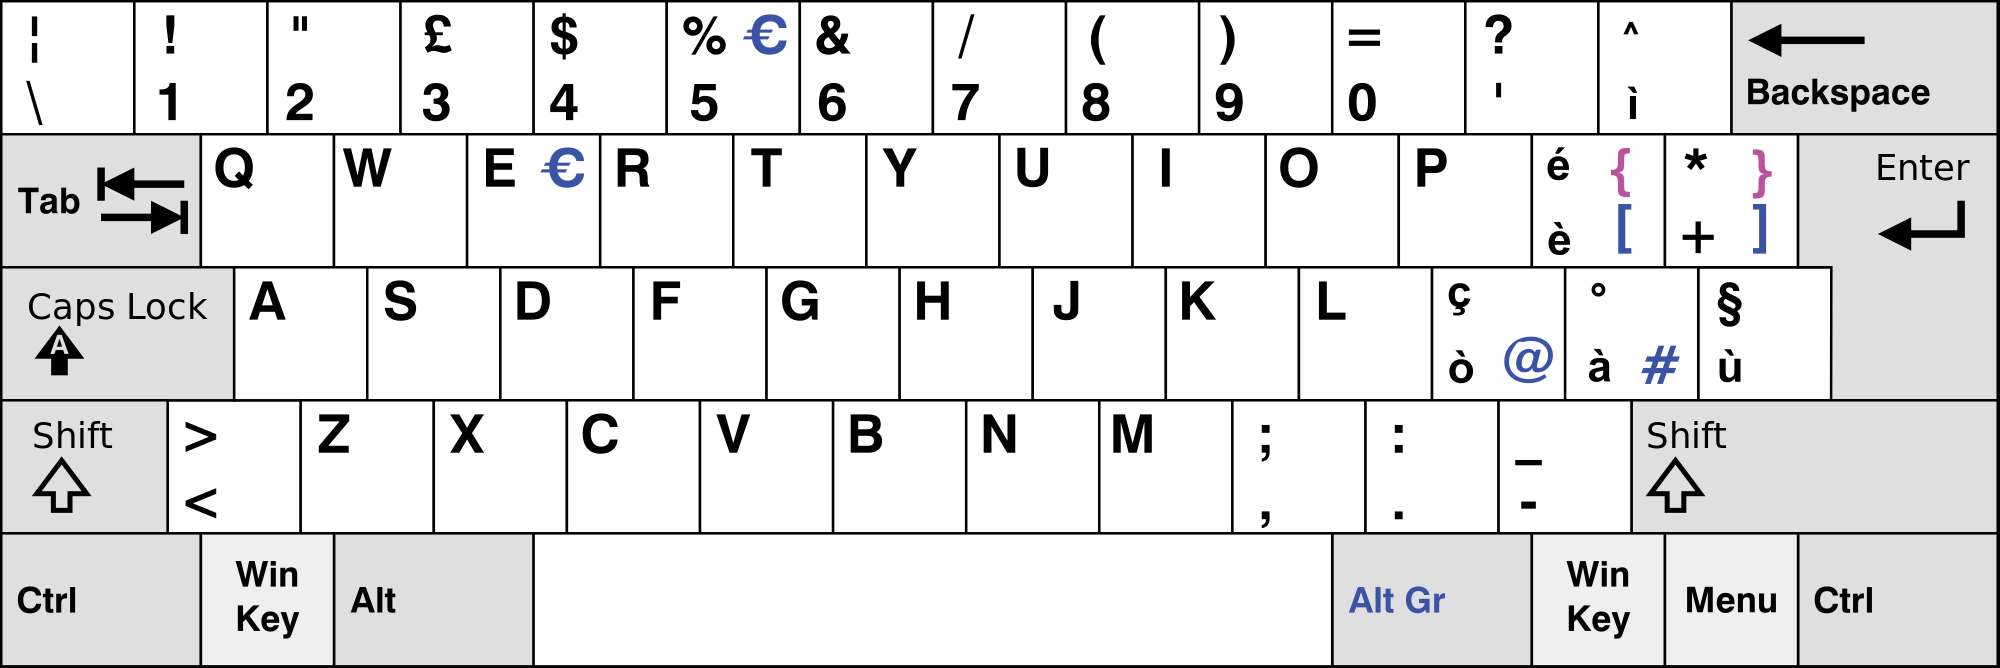
\includegraphics[width=\textwidth]{images/qwerty.png}
        \caption{Qwerty-based layout}
    \end{subfigure}
	 \begin{subfigure}[b]{0.3\textwidth}
        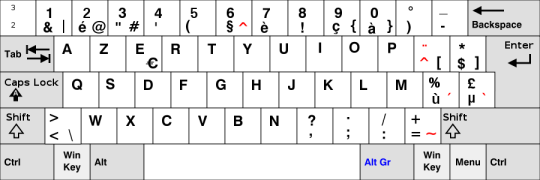
\includegraphics[width=\textwidth]{images/azerty.png}
        \caption{Azerty-based layout}
    \end{subfigure} 
    \begin{subfigure}[b]{0.3\textwidth}
        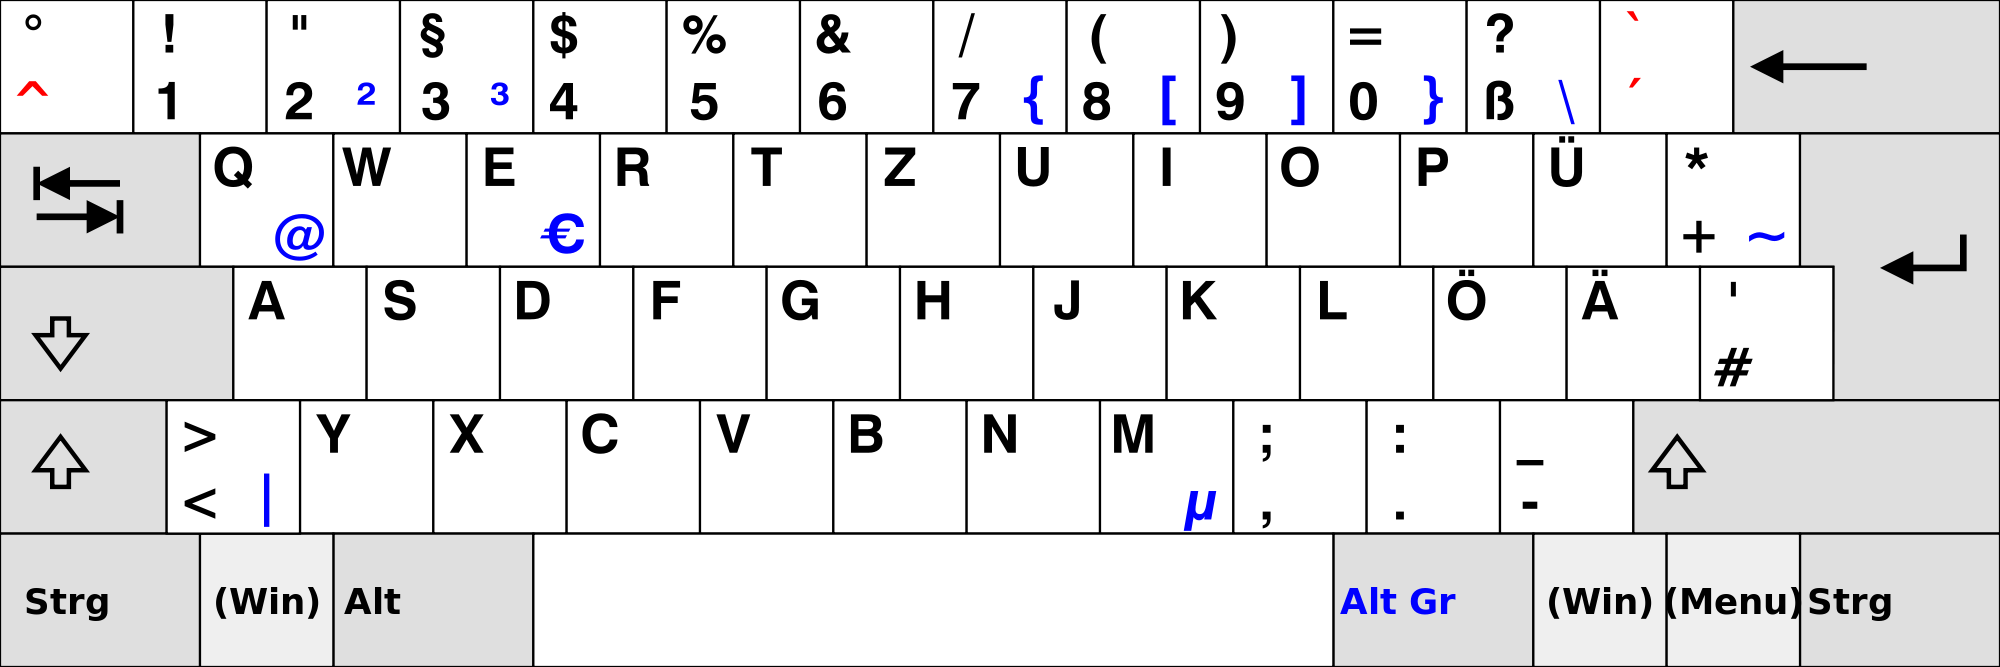
\includegraphics[width=\textwidth]{images/qwertz.png}
        \caption{Qwertz-based layout}
    \end{subfigure}
    \caption{Most common layouts in Europe}
\end{figure}
\clearpage

\section{Practice}
The more you know, the more you type. Once you are able to type a full word one needs to keep practising. This builds up a muscle memory of all the possible key stokes which make up the words of the dictionary.
The computerhope.com\citep{computerhope} website provide good everyday practice example to follow. There is also a large collection of games on the internet to practice and therefore improve the typing speed.\\
how-to-type.com \cite{howto} offers practice sessions such as 10 minutes to an hour per session as their recommendation.
The book written by \citet{handBook} also gives some advice regarding the finger position and the stretch to do beforehand.
There is no software which combines both, doing a check that the user has done finger stretches, and provide advice on how to position yourself in front of the keyboard improving your ability to type correctly. Each of these is done on an individual basis.

\section{Speed and accuracy}
Accuracy is the first skill we need to develop (typing for beginners)\cite{beginners}.\\
Firstly, the user must learn how to type all the letters of the keyboard, as said above. The user must know the exact position of each letter on the keyboard, without having to look at it. Once they know this, they will have the ability to type much faster. However faster can also mean more mistakes. If the mistake is found on the same letter, the user must practice typing this letter again and again to improve accuracy. The problem can also come from a finger which is not reactive enough. In this case, steps need to be put in place in order to train that particular finger. This will be one of the goals of the software to be created. Also, the user must be aware that the more improvement regarding typing speed, the harder it will become to improve this speed.(lingholic.com) \cite{plateau}. Below are two graphs explaining the difference between the expected learning curve and the actual learning curve.

\begin{figure}[H]
    \centering
    \begin{subfigure}[b]{0.4\textwidth}
        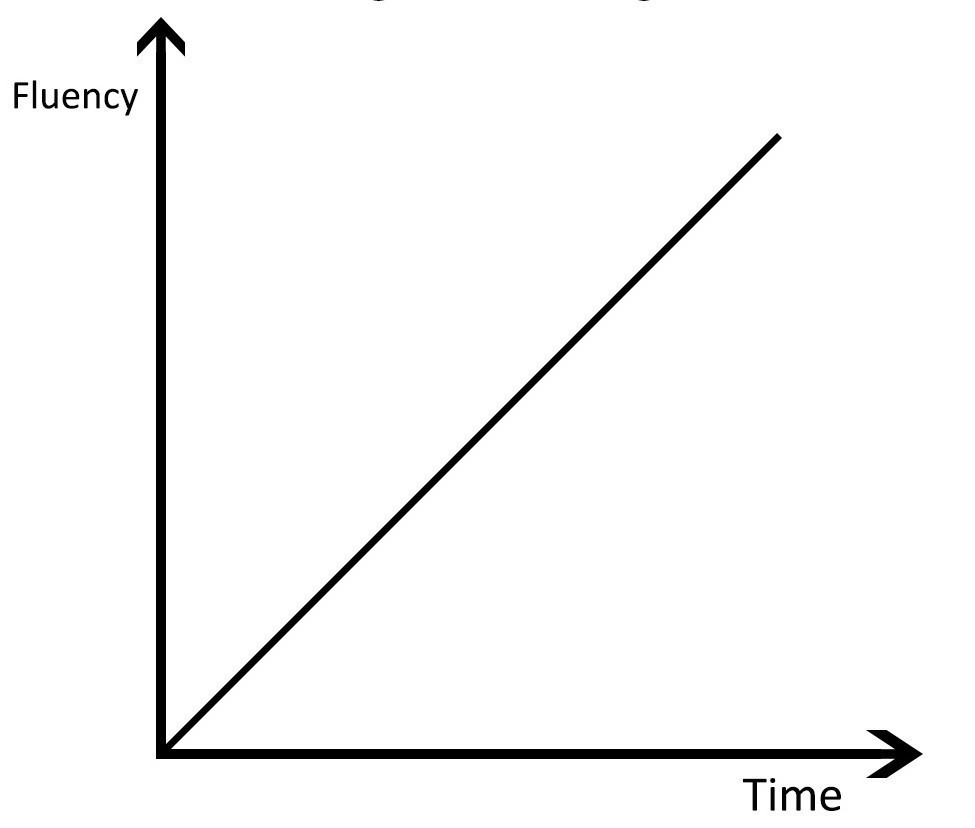
\includegraphics[width=\textwidth]{images/expected.jpg}
        \caption{Expected learning curve}
    \end{subfigure}
    \begin{subfigure}[b]{0.4\textwidth}
        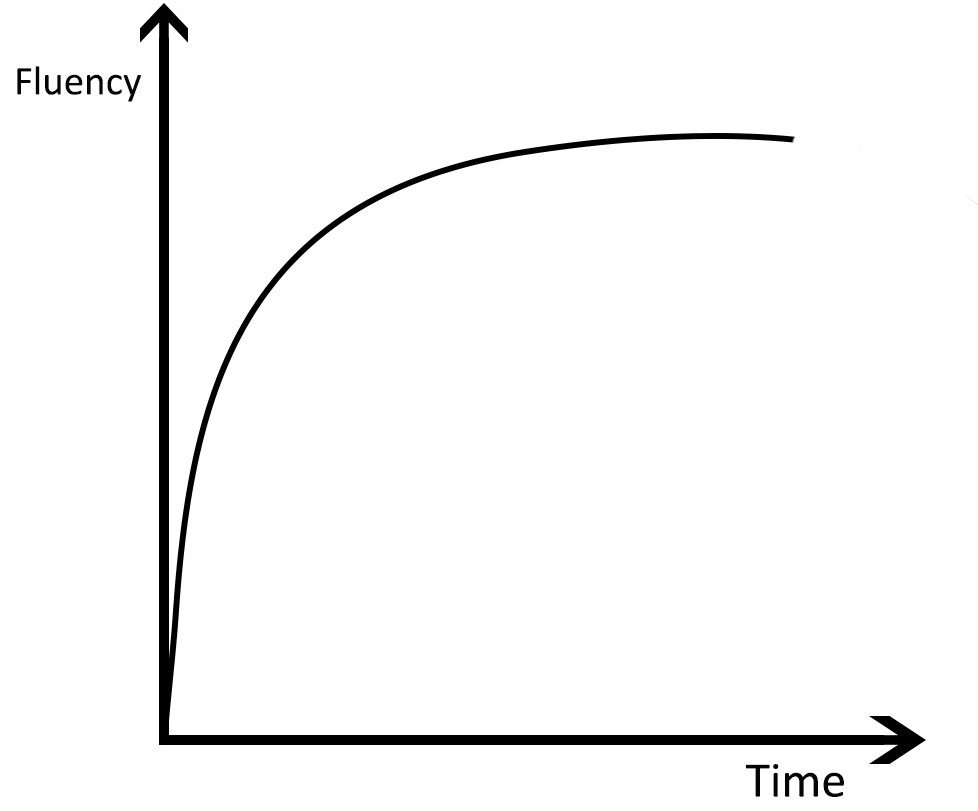
\includegraphics[width=\textwidth]{images/actual.jpg}
        \caption{Actual learning curve}
    \end{subfigure}
    \caption{Expected and actual learning curve}
\end{figure}

\clearpage
\chapter{Conclusion}
From the current knowledge in typing, it appears that it is possible to quickly easily to learn to type faster and with a good accuracy. It is important for the user to learn the basics of the keyboard and the position of the letters. Once this is known, with the time and practice, typing speed will slowly and steadily increase.\\
Whenever the user has some accuracy problem with a single finger, practice will increase general precision.\\
For the general public, it they have a computer and a keyboard, they can learn how to type faster in three steps :
\begin{itemize}
	\item Learn the position of the letters on the keyboard and associate each fingers to each key
	\item Practice in order to improve the speed
	\item Correct the accuracy problems
\end{itemize}

\clearpage

%Bibliography
\begin{flushleft}
	\bibliographystyle{unsrtnat}
	\bibliography{lit_review.bib}
\end{flushleft}

\clearpage
\afterpage{\blankpage}

\end{document}